\chapter{Applicability to Amputee Data}
\label{chp:amputee-data}

The collection of labelled training data is ardours, this becomes more acute when the subject has restricted movement such as for an amputee. Therefore any system which can reduce the data requirements for these individuals is of benefit. In Chapter \ref{chp:personalisation} methods for personalisation of a machine learning model using additional data from other subjects were demonstrated to both improve the performance of a model and reduce the data requirements for that model. Within this chapter these methods will be implemented for an amputee to investigate it they are applicable to someone with a substantially different gait to the normal population.

Within this chapter we will investigate whether the personalisation methods developed in Chapter \ref{chp:personalisation} can use prior non-amputee data to improve the performance of an \acrshort{lmr} classifier for an individual amputee.

The contributions of this Chapter are:
\begin{itemize}
    \item Collection of amputee gait data that is directly comparable to non-amputee data
    \item Comparison of shank \acrshort{imu} data between non-amputee, intact limb and prosthetic
    \item Demonstration of performance differences of \acrshort{lmr} network of intact and prosthetic side
    \item Demonstration of transfer learning from non-amputee data to an amputee for \acrshort{marg} gait data
\end{itemize}

% Sometimes an overview of the chapter
First related works are presented. This is followed by Section \ref{sec:amputee-methods} in which an explanation of the methods used and presentation of amputee data collected are provided. Following this the results of a baseline model performance, and performance of two personalisation methods in Sections \ref{sec:amputee-baseline}, \ref{sec:amputee-supplementation} and \ref{sec:amputee-transfer} respectively. Finally discussion and conclusion are given in Section \ref{sec:amputee-discussion}.


%-----------------------------------------------------------------
\section{Related Works}
\label{sec:amputee-related-works}
The gait of a lower-limb amputee varies dramatically between individuals\cite{Lonini2016} often presenting asymmetrically\cite{Roerdink2012}. This asymmetry is seen in many gait features including stance and swing periods, and hip, knee and ankle joint moments\cite{Adamczyk2015, Harandi2020}. A common explanation for this is the reduced push-off capacity of the prosthetic leg, but it may also be due to discomfort of the prosthetic\cite{Hak2014}. Many lower limb amputees attempt to maximise the capacities of their intact limb to counteract the limitations of their prosthetic device\cite{Ochoa-Diaz2020}. This asymmetry results is a substantially different gait from the norm. Therefore techniques that work for non-amputees are not necessarily directly applicable to amputees or other gait impairments\cite{Jamieson2021}.

Lonini et al considered a personal model trained from a target's data was required. Or if a global model from other patients was all that was required. The study involved the classification of physical activities based on sensor data from a waist worn accelerometer.  Eleven non-amputee and ten patients who use an Knee-Ankle-Foot Orthotic (KAFO) device were asked to perform five actions. There work suggested that models trained exclusively of subject without gait impairments performed poorly when tested using the KAFO subjects. However the model trained from only KAFO subjects performed only slightly worse than the personalised baseline.\cite{Lonini2016}

Jamieson et al performed a study comparing the performance of supervised classifiers for both amputee and non-amputee carrying out the same activities. Data collected was collected from a hip mounted \acrshort{imu} with participants asked to walk an improvised route in the vicinity of their homes. A both \acrfull{svm} and \acrshort{lstm} networks were trained to classify different locomotive activities. Classifiers were trained with varying sets of data constructed by \acrfull{looxv}. Several configurations of subjects were tested. Most notable a network was trained using exclusively non-amputee data but tested using amputees data. Classification accuracy fell $~78\%$ for non-amputees to an average of $~55\%$ for the four amputees. Jamieson concluded that classifiers trained using exclusive persons without gait impairments would not be suitable for those with impaired gait.\cite{Jamieson2021}

Gao et al presented work investigating Reinforcement Learning (RL) schemes for controlling a lower limb prosthesis that was personalised to an individual. They first collected data from two non-amputees wearing a below knee prosthetic device. This data was used to generate base knowledge that could be used as a starting point for their RL scheme. Using the human locomotive simulator OpenSim they implemented models of amputee gaits. These were then use to demonstrate a RL scheme that could adapt to an individual.\cite{Gao2020a}

There is only limited literature on applying classifiers built from non-amputee data to amputations. The literature that exists suggest that in order to achieve adequate classification accuracy the gait abnormalities of an amputee must be taken into account. The personalisation methods developed in the previous chapter appear to be a good fit for problem.

From the literature surveyed the following gaps were identified:
\begin{itemize}
    \item No work has attempted to use transfer learning to personalise a non-amputee \acrshort{lmr} model for an amputee
    \item No papers have investigated the difference in classification performance between amputated and in-tact limb
\end{itemize}

The remainder of this chapter will focus on investigating these gaps.

%-----------------------------------------------------------------
\section{Methods and Materials}
\label{sec:amputee-methods}
% Recap methods and what has changed
The methods used in this chapter will mirror those used in previous chapters. Additional data for an amputee was collected. This was used to generate a new set of baselines to compare the results of the personalisation methods previously developed against. Full tables of results for all experiments can be found in  Appendix \ref{chp:tables-of-results} Section \ref{sec:app-a-amputee-transfer-learning}.

Data was collected from a single left trans-tibial amputee wearing a Blatchford Echelon VT prosthetic limb. The data was collected by Blatchford Product Limited. The data was collected in the same manner as previously described, however a clinician at the centre held the smartphone to annotate activities in order to reduce the fall risk for the amputee. Table \ref{tab:summary-of-episode-amputee-data} shows a summary of the data collected including the number of data samples and the number of episode for each activity.

\begin{table}[hbt]
    \centering
    \caption{Summary of amputee gait data collected}
    \label{tab:summary-of-episode-amputee-data}
    \begin{tabularx}{\textwidth}{c *{6}{Y}}
        \noalign{\hrule height 1.5pt}
        \textbf{Activity} & WALK & \glsentryshort{ra} & \glsentryshort{rd} & \glsentryshort{sa} & \glsentryshort{sd} & STOP \\
        \hline
        \textbf{Samples} & 38114 & 6159 & 7194 & 2872 & 2450 & 11763 \\
        \textbf{Episodes} & 26 & 7 & 7 & 4 & 4 & 15 \\
        \noalign{\hrule height 1.5pt} \\
    \end{tabularx}
\end{table}

\begin{table}[hbt]
    \centering
    \begin{tabular}{c|c}
         &  \\
         & 
    \end{tabular}
    \caption{Add picture of Kelvin}
    \label{tab:my_label}
\end{table}

As significantly less data is available to test with, adjustments had to be made the quantities used in each of the data sets. The test data set was reduced from 5000 windows to 250 windows. The range of training windows tested was reduced to between 100 and 750. Additionally in order to ensure that there was sufficient episodes for \acrshort{sa} and \acrshort{sd} each of the stair episodes was split up into new episodes containing a maximum of 200 samples each. This increased the number of available episode to episodes for both stair activities. 

Due to asymmetry the left and right ankle data cannot be combined. This will be described further in the following section. All other quantities and hyper-parameters remained the same.

\subsection{Amputee Gait Data}
Gait asymmetry of amputees means that unlike in the previous chapter the left and right ankle data cannot be combined to increase the dataset size. Instead both sides will be evaluated independently to investigate the performance differences between the side. Figure \ref{fig:ch6_amputee_gyro_trends} shows the angular velocity of the shank in the Saggital plane for the intact and prosthetic limbs of a left amputated trans-tibial amputee. The left ankle has been transformed using Equation \ref{eqn:left-right-transformation} so both ankles are presented in the same axes. For comparison the ankle angular velocity of the non-amputee subject 1 is shown.

% How does it differ from non-amputee gait data
\begin{figure}[p]
    \begin{tabular}{lccc}
        & \textbf{Non-Amputee} & \textbf{Amputee -- Intact Limb} & \textbf{Amputee -- Prosthetic} \vspace{0.2cm}\\

        \rotatebox{90}{\enspace\qquad \textbf{Walking}} &
        \begin{subfigure}[b]{0.275\textwidth}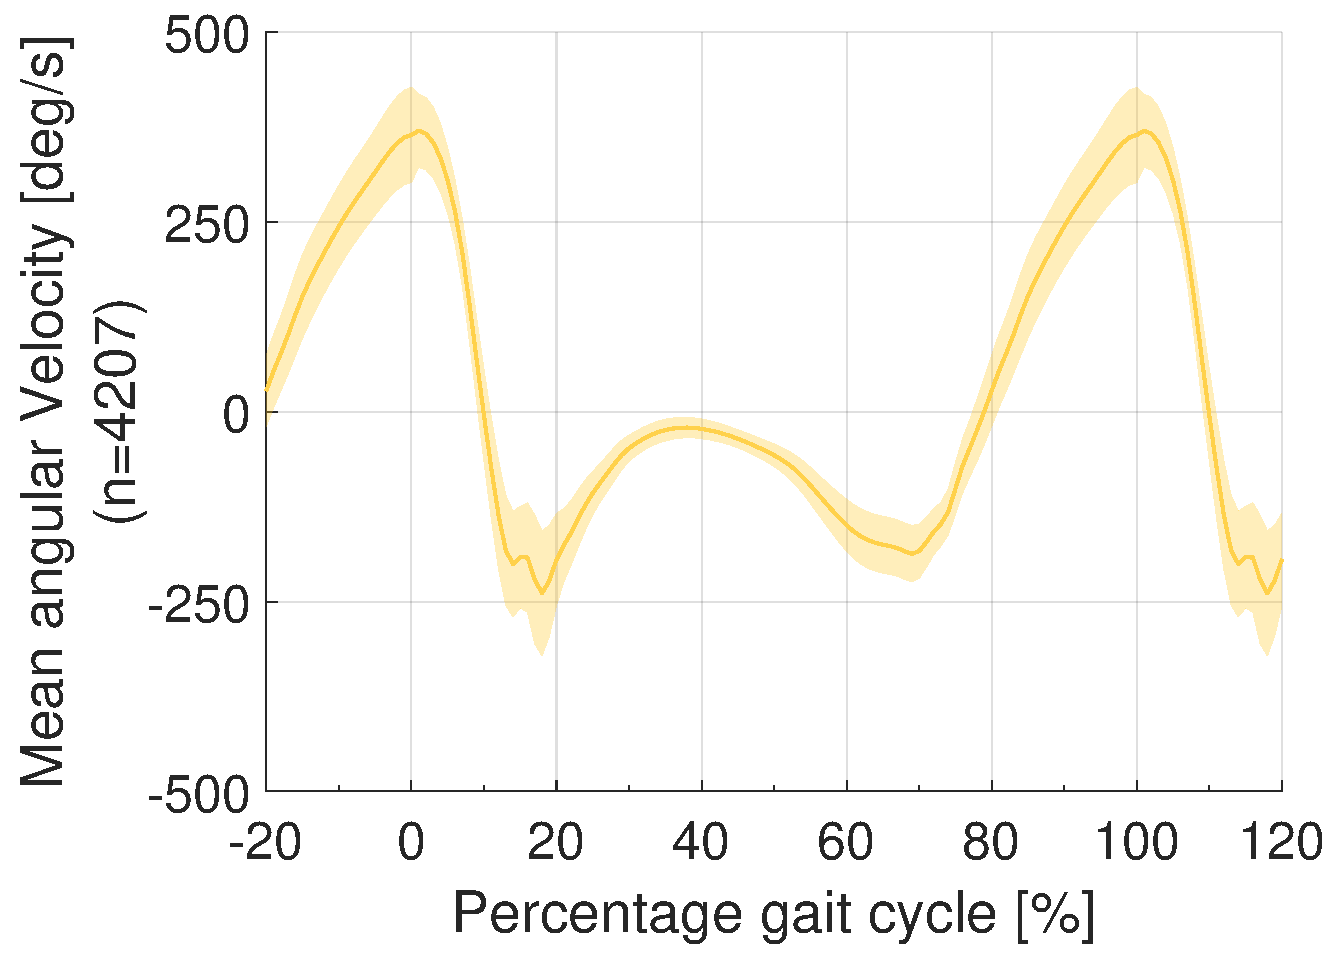
\includegraphics[width=\linewidth]{content/6-Amputee/Gait-Trends/ch6_subject_01_gait_trends_r_ankle_gyro_z_activity_walking.pdf}\end{subfigure} & \begin{subfigure}[b]{0.275\textwidth}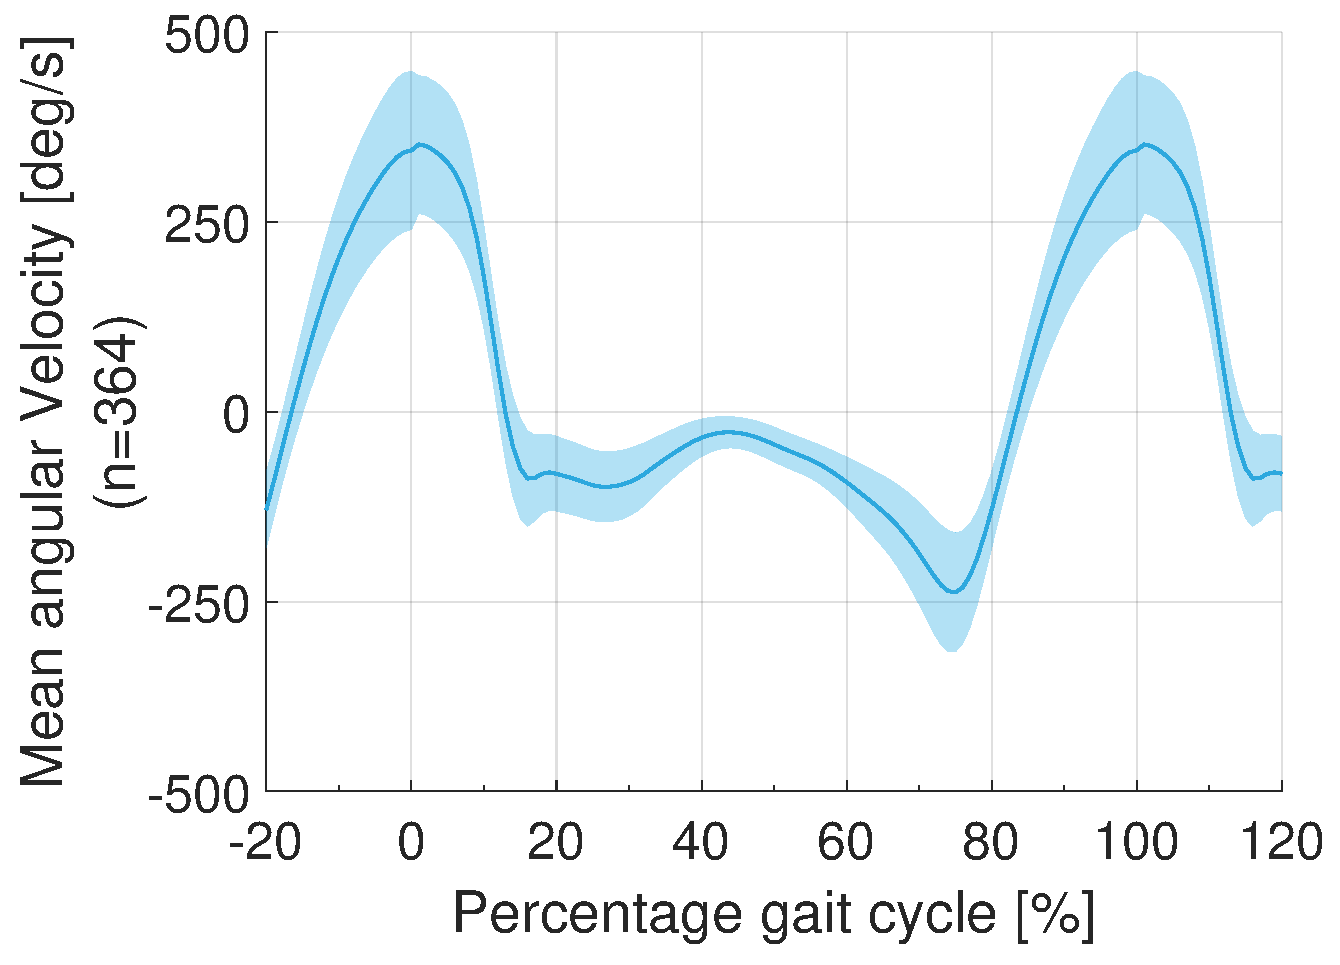
\includegraphics[width=\linewidth]{content/6-Amputee/Gait-Trends/ch6_amputee_gait_trends_l_ankle_gyro_z_activity_walking.pdf}\end{subfigure} &
        \begin{subfigure}[b]{0.275\textwidth}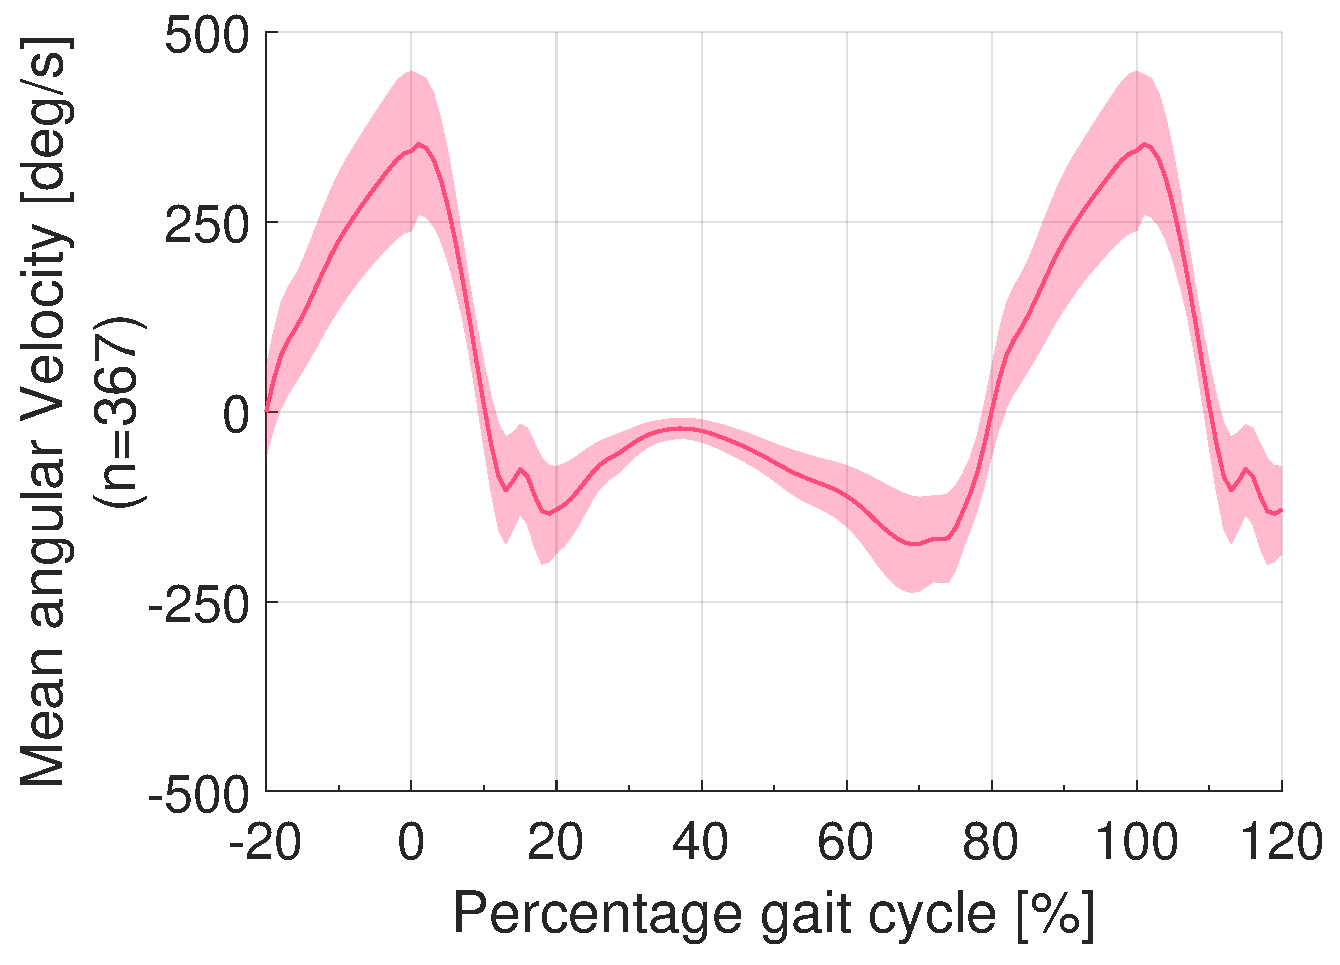
\includegraphics[width=\linewidth]{content/6-Amputee/Gait-Trends/ch6_amputee_gait_trends_r_ankle_gyro_z_activity_walking.pdf}\end{subfigure} \\
        
        \rotatebox{90}{~\quad \textbf{Ramp Ascent}} & 
        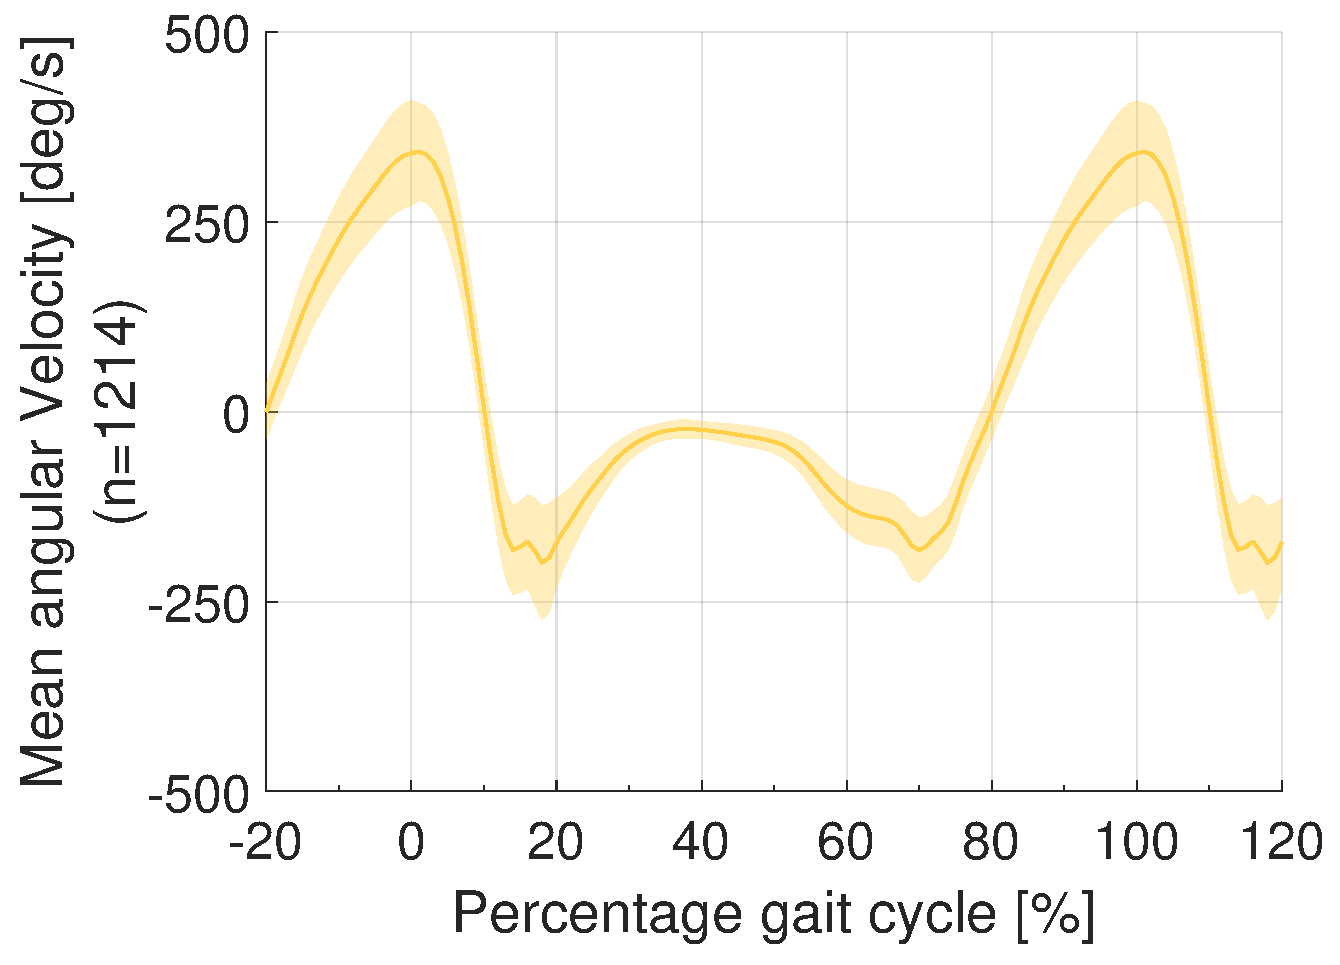
\includegraphics[width=0.275\linewidth]{content/6-Amputee/Gait-Trends/ch6_subject_01_gait_trends_r_ankle_gyro_z_activity_ramp_up.pdf} & 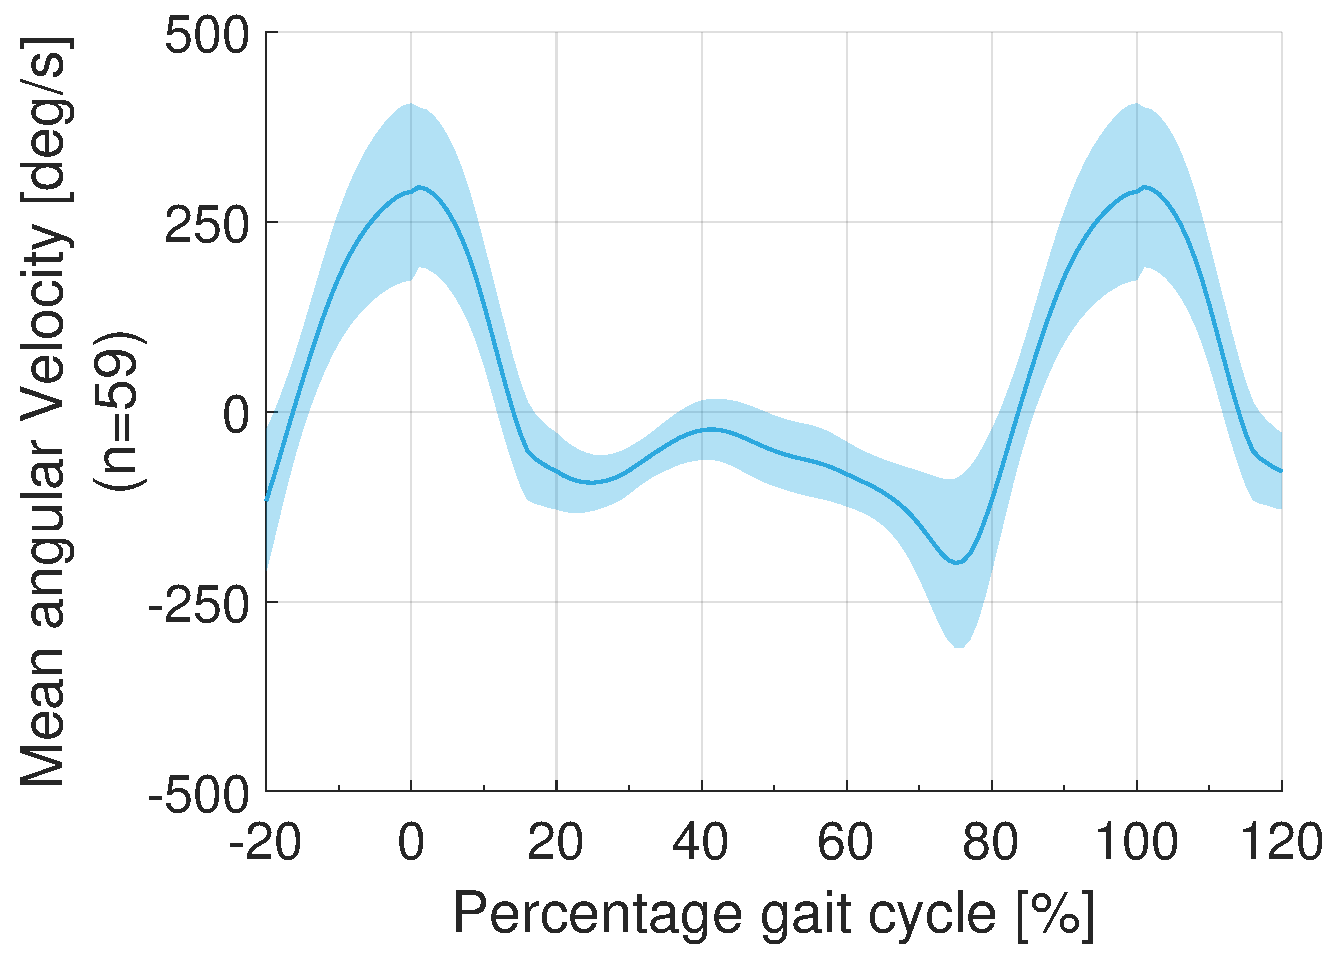
\includegraphics[width=0.275\linewidth]{content/6-Amputee/Gait-Trends/ch6_amputee_gait_trends_l_ankle_gyro_z_activity_ramp_up.pdf} &
        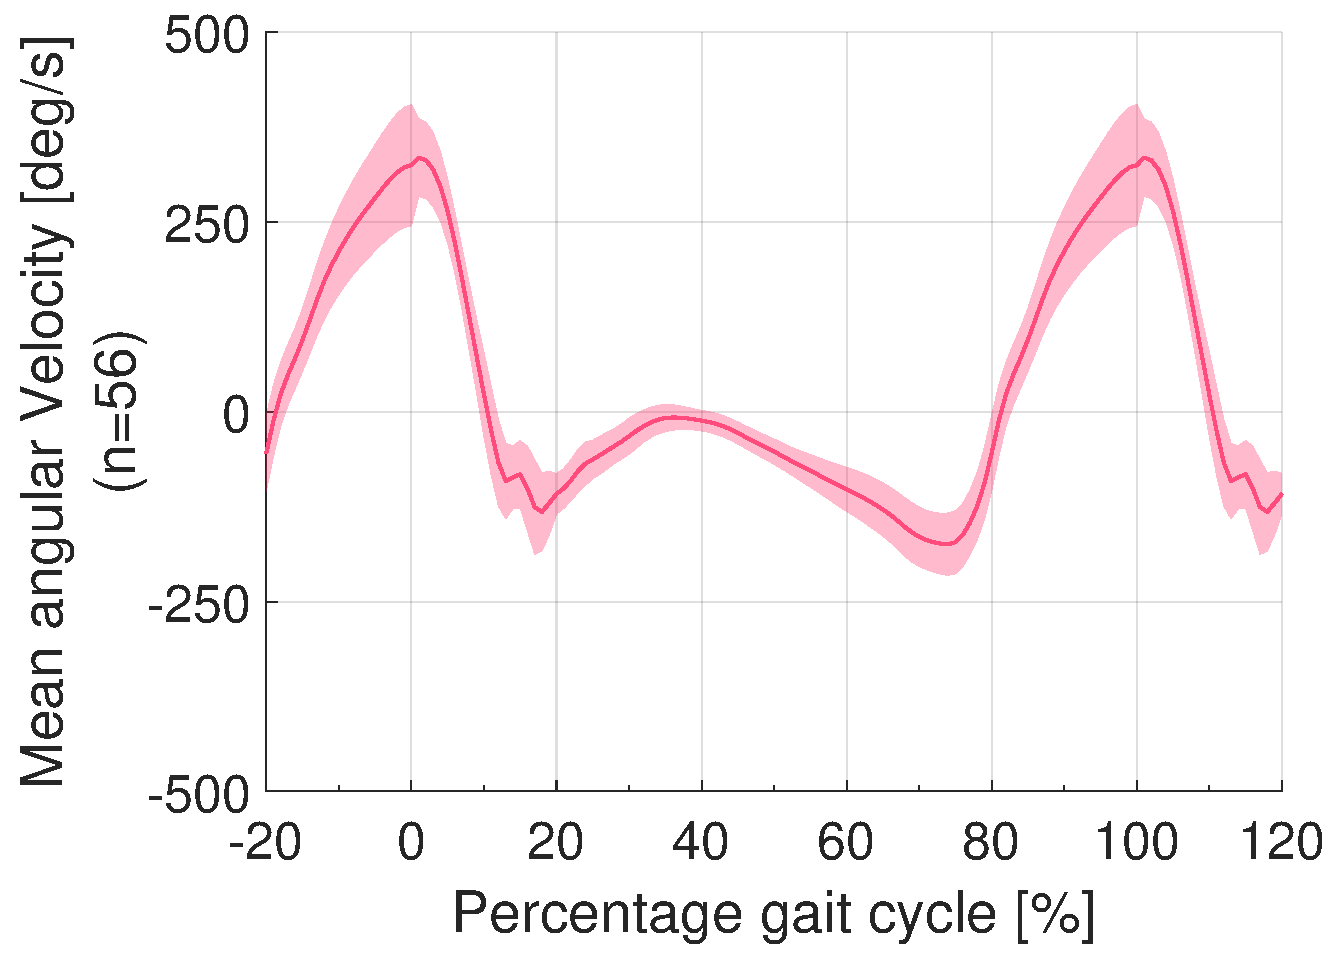
\includegraphics[width=0.275\linewidth]{content/6-Amputee/Gait-Trends/ch6_amputee_gait_trends_r_ankle_gyro_z_activity_ramp_up.pdf} \\
        
        \rotatebox{90}{\quad \textbf{Ramp Descent}} & 
        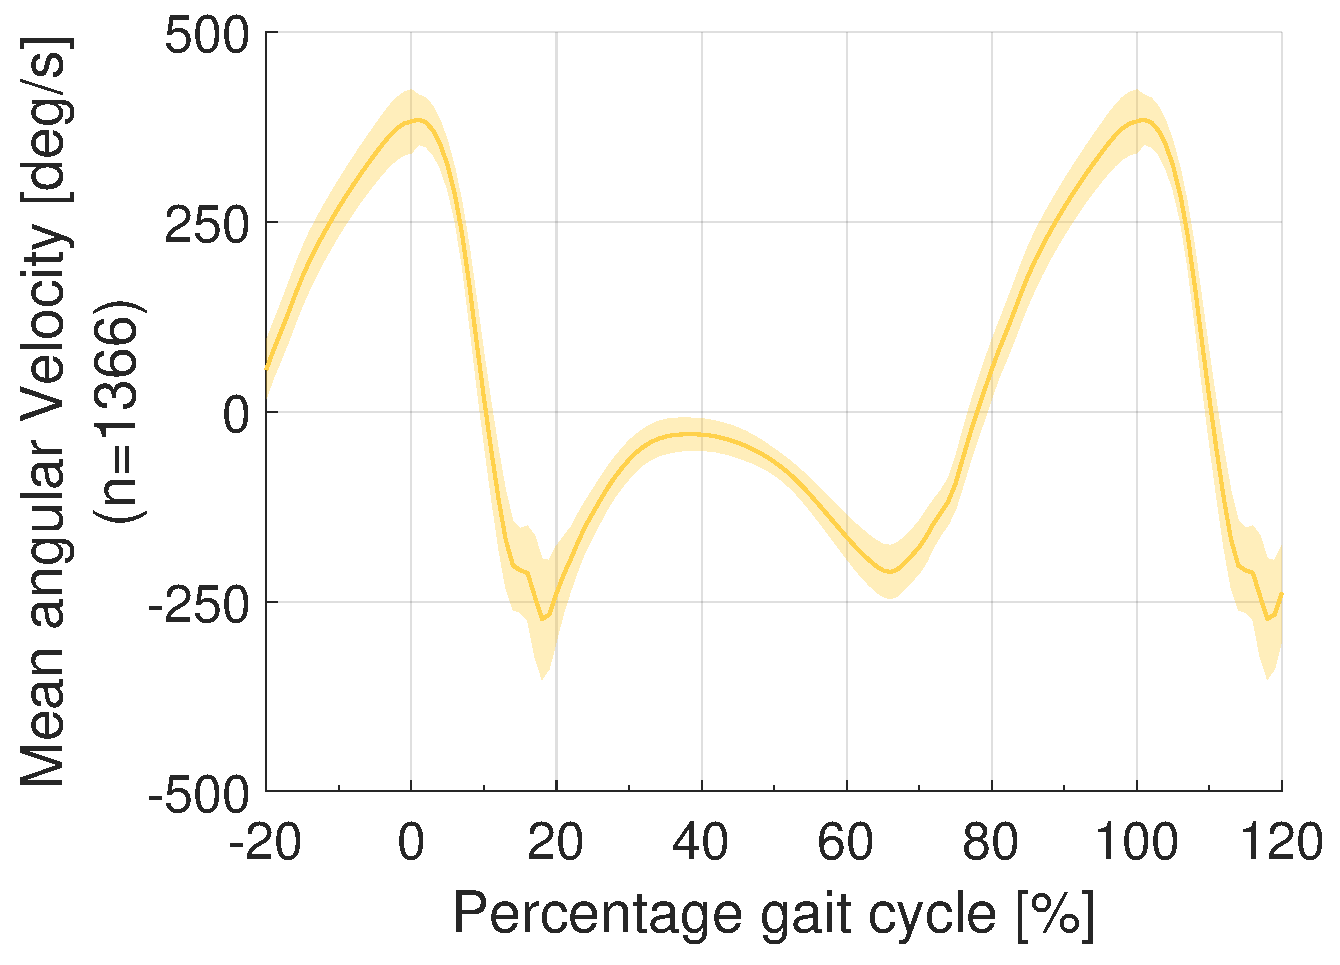
\includegraphics[width=0.275\linewidth]{content/6-Amputee/Gait-Trends/ch6_subject_01_gait_trends_r_ankle_gyro_z_activity_ramp_down.pdf} & 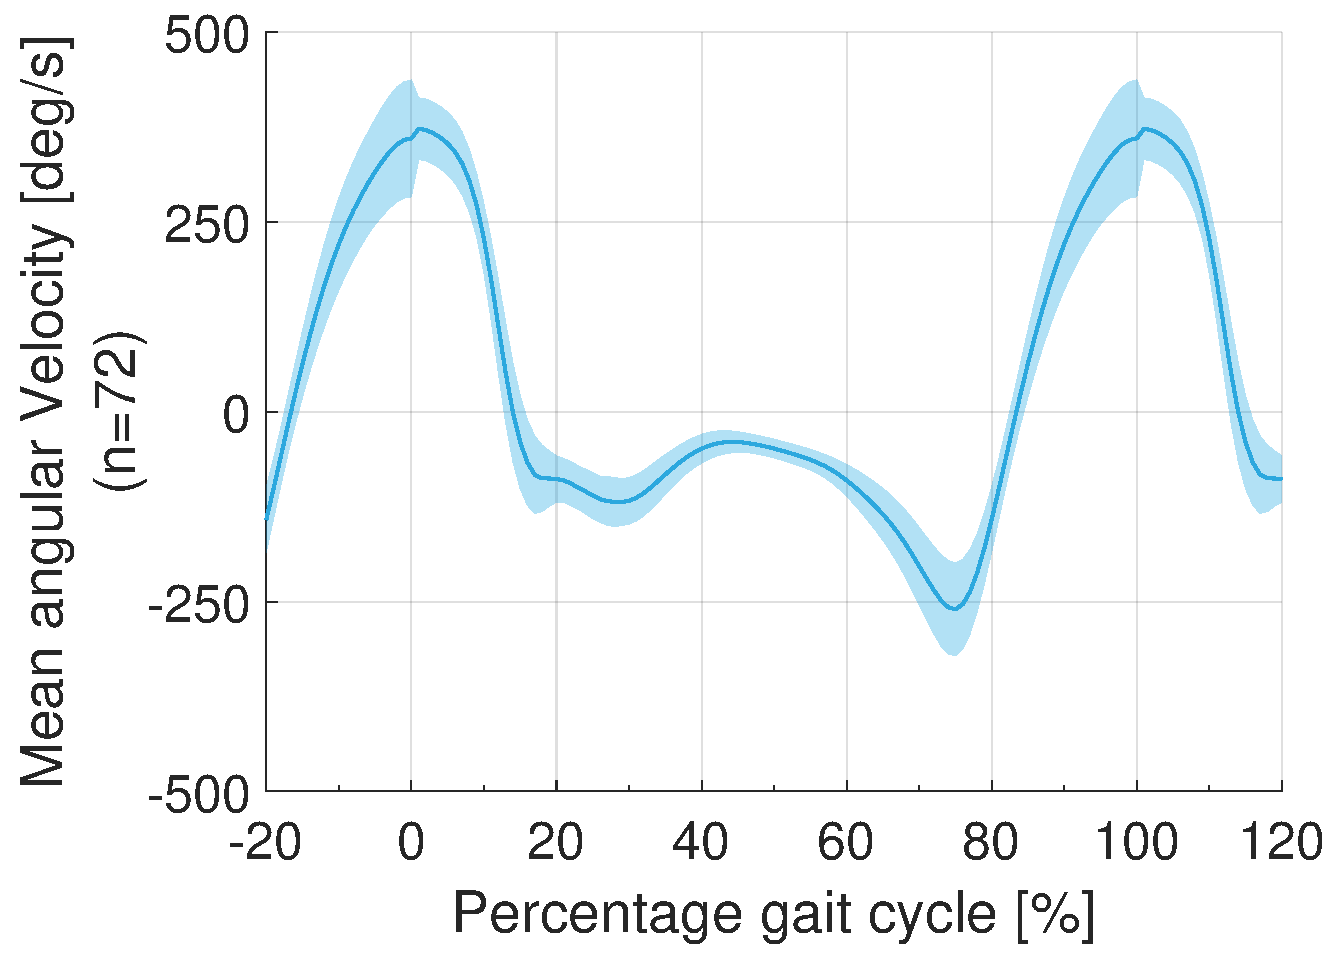
\includegraphics[width=0.275\linewidth]{content/6-Amputee/Gait-Trends/ch6_amputee_gait_trends_l_ankle_gyro_z_activity_ramp_down.pdf} &
        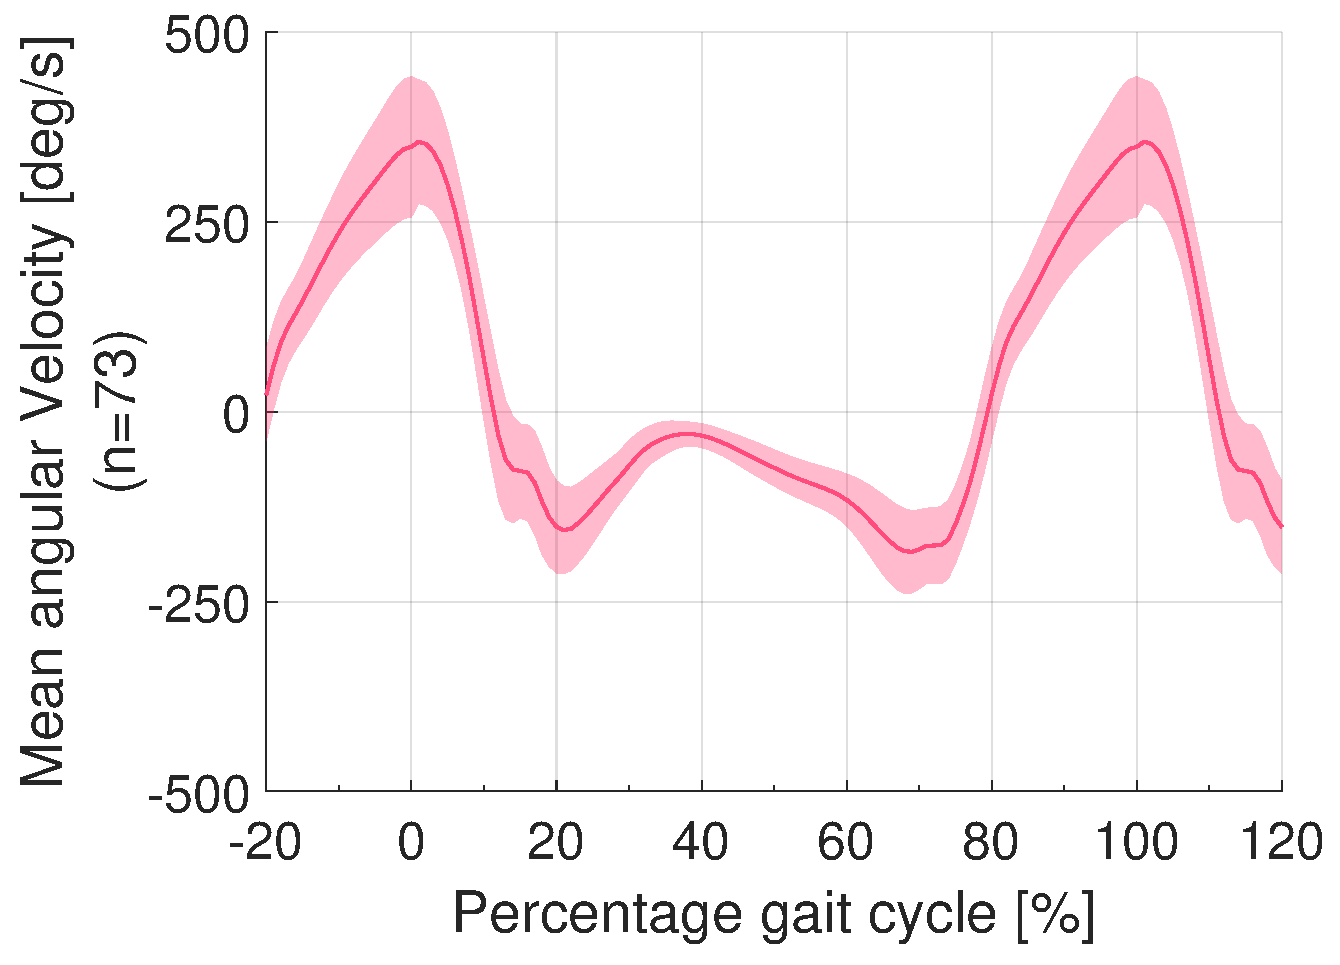
\includegraphics[width=0.275\linewidth]{content/6-Amputee/Gait-Trends/ch6_amputee_gait_trends_r_ankle_gyro_z_activity_ramp_down.pdf} \\
        
        \rotatebox{90}{~\quad \textbf{Stair Ascent}} & 
        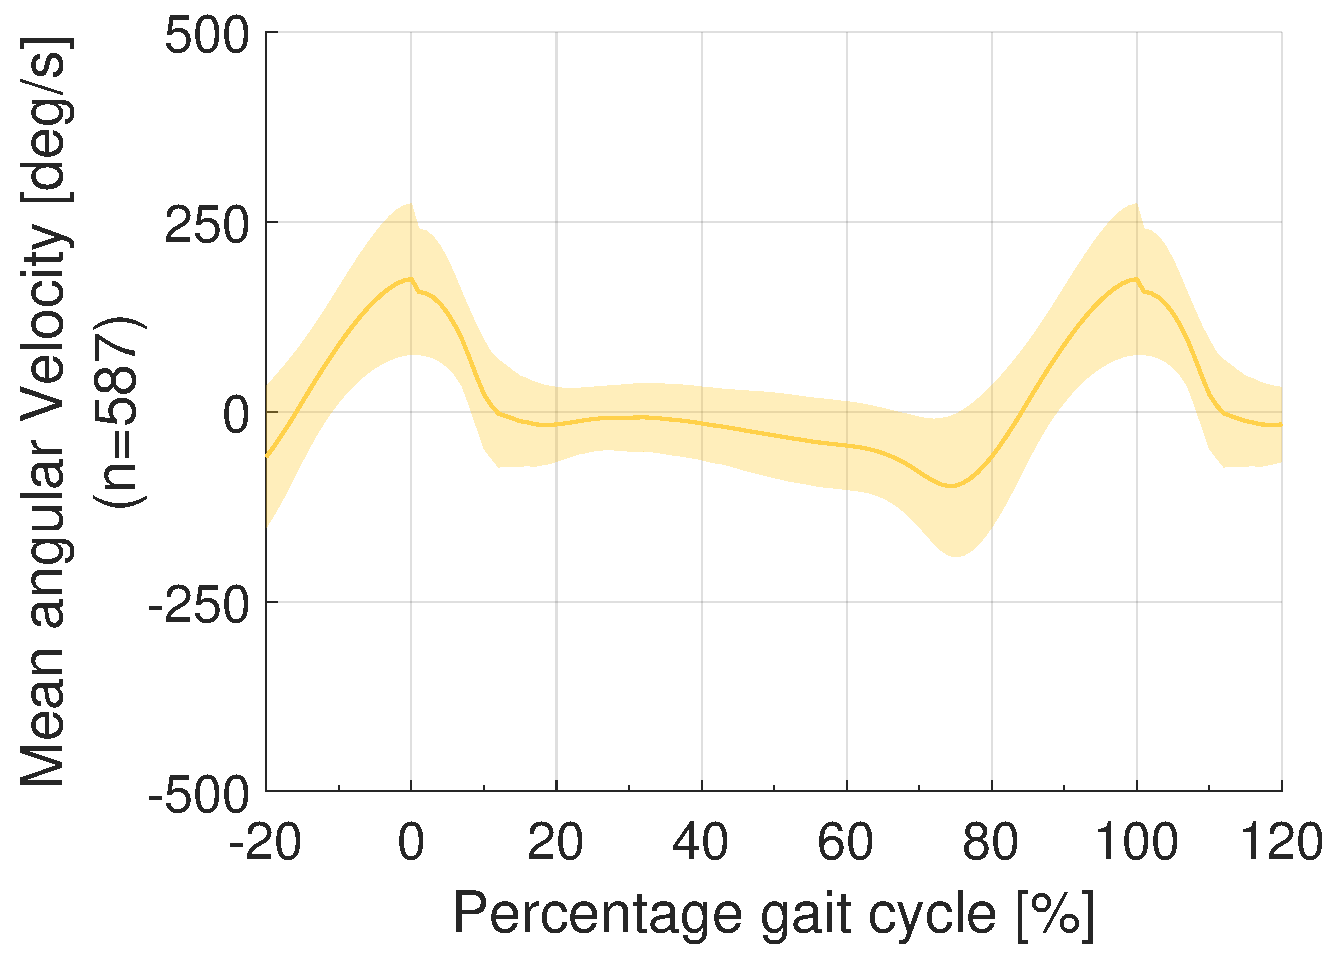
\includegraphics[width=0.275\linewidth]{content/6-Amputee/Gait-Trends/ch6_subject_01_gait_trends_r_ankle_gyro_z_activity_stair_up.pdf} & 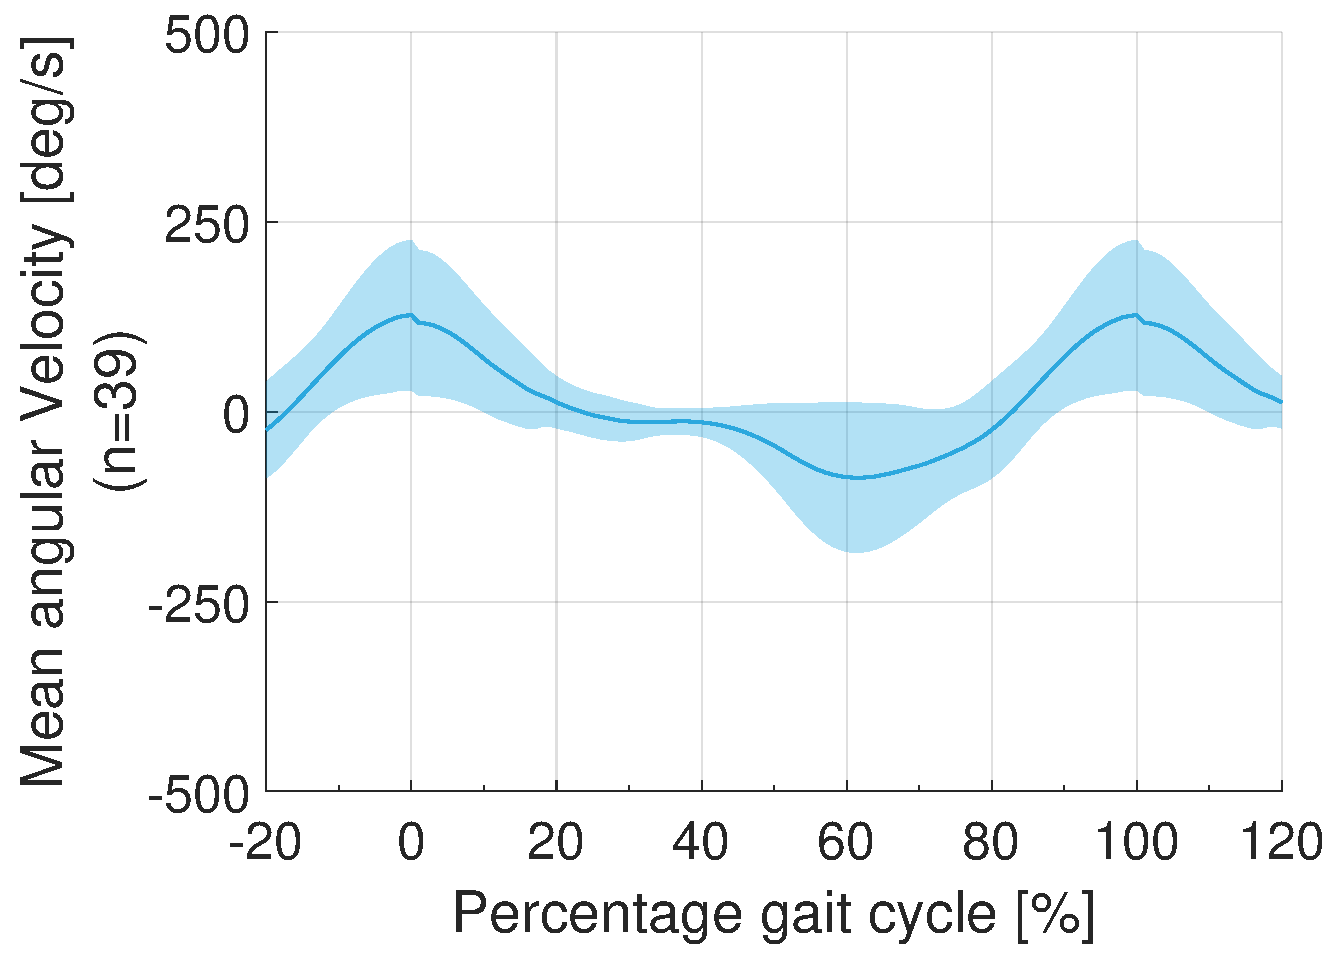
\includegraphics[width=0.275\linewidth]{content/6-Amputee/Gait-Trends/ch6_amputee_gait_trends_l_ankle_gyro_z_activity_stair_up.pdf} &
        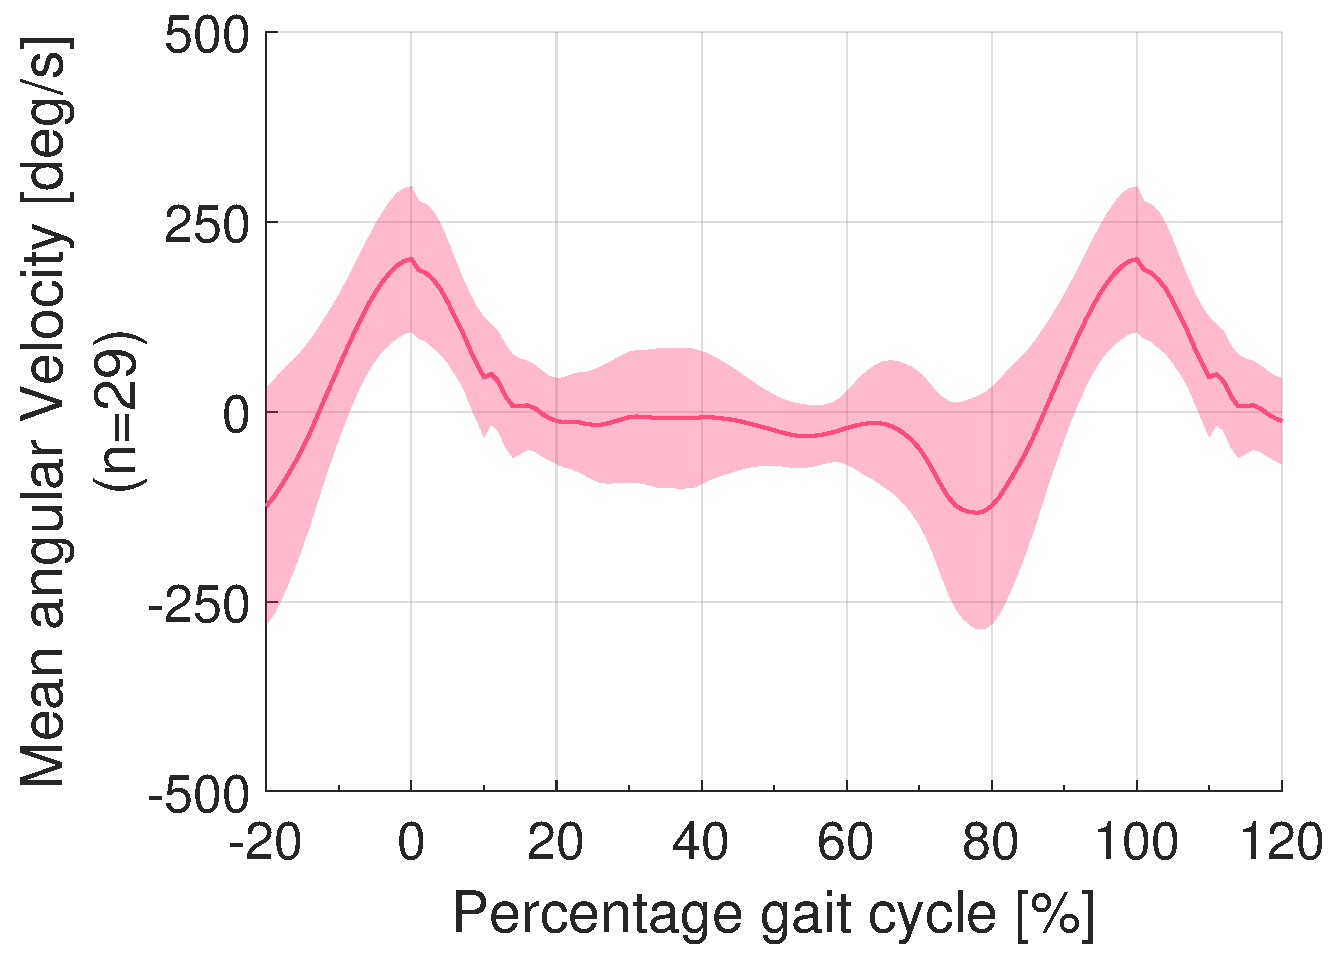
\includegraphics[width=0.275\linewidth]{content/6-Amputee/Gait-Trends/ch6_amputee_gait_trends_r_ankle_gyro_z_activity_stair_up.pdf} \\
        
        \rotatebox{90}{\quad \textbf{Stair Descent}} & 
        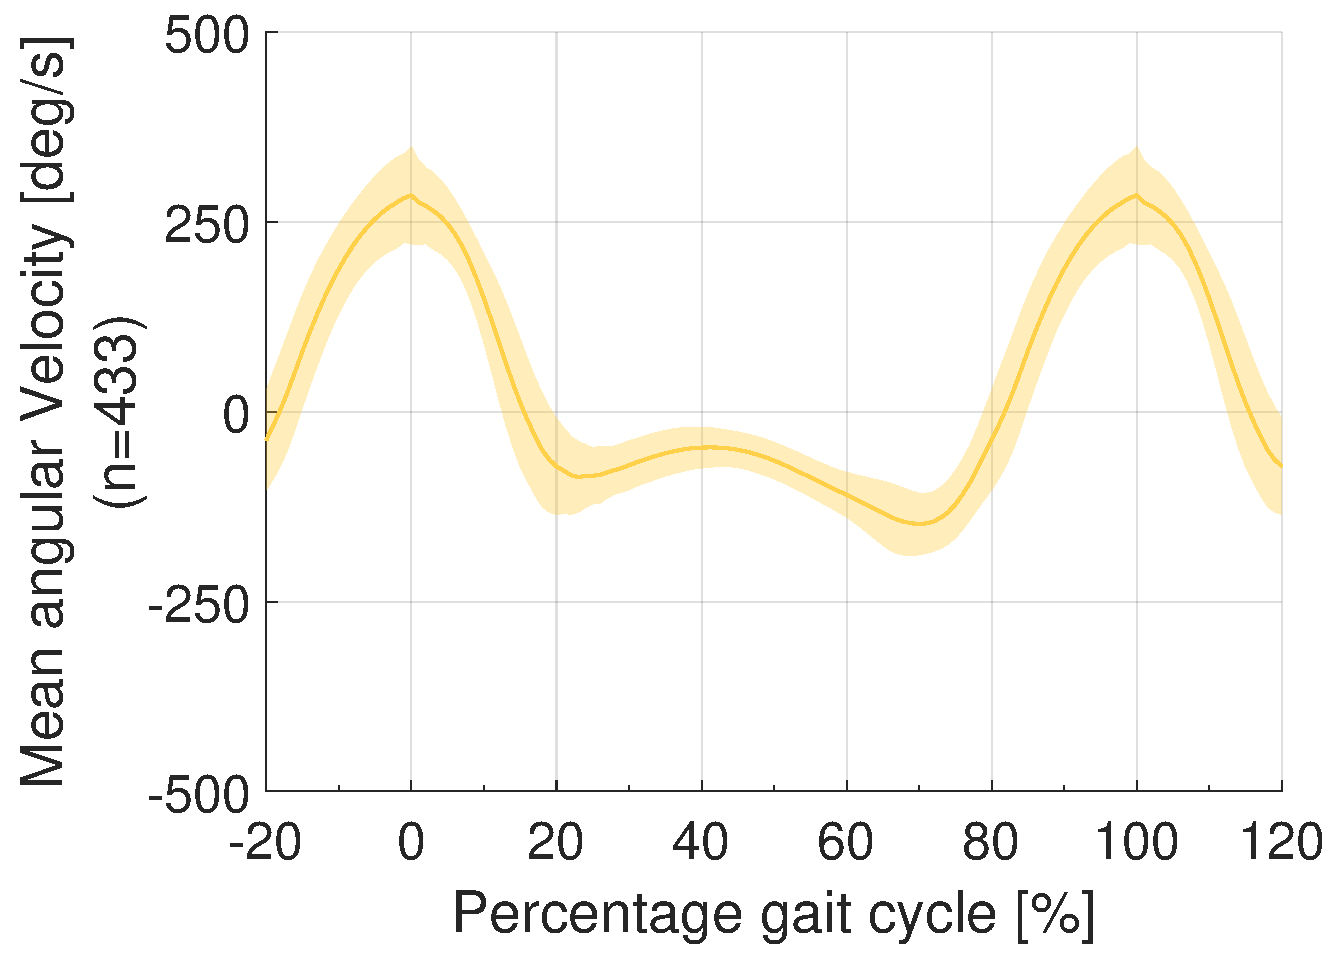
\includegraphics[width=0.275\linewidth]{content/6-Amputee/Gait-Trends/ch6_subject_01_gait_trends_r_ankle_gyro_z_activity_stair_down.pdf} & 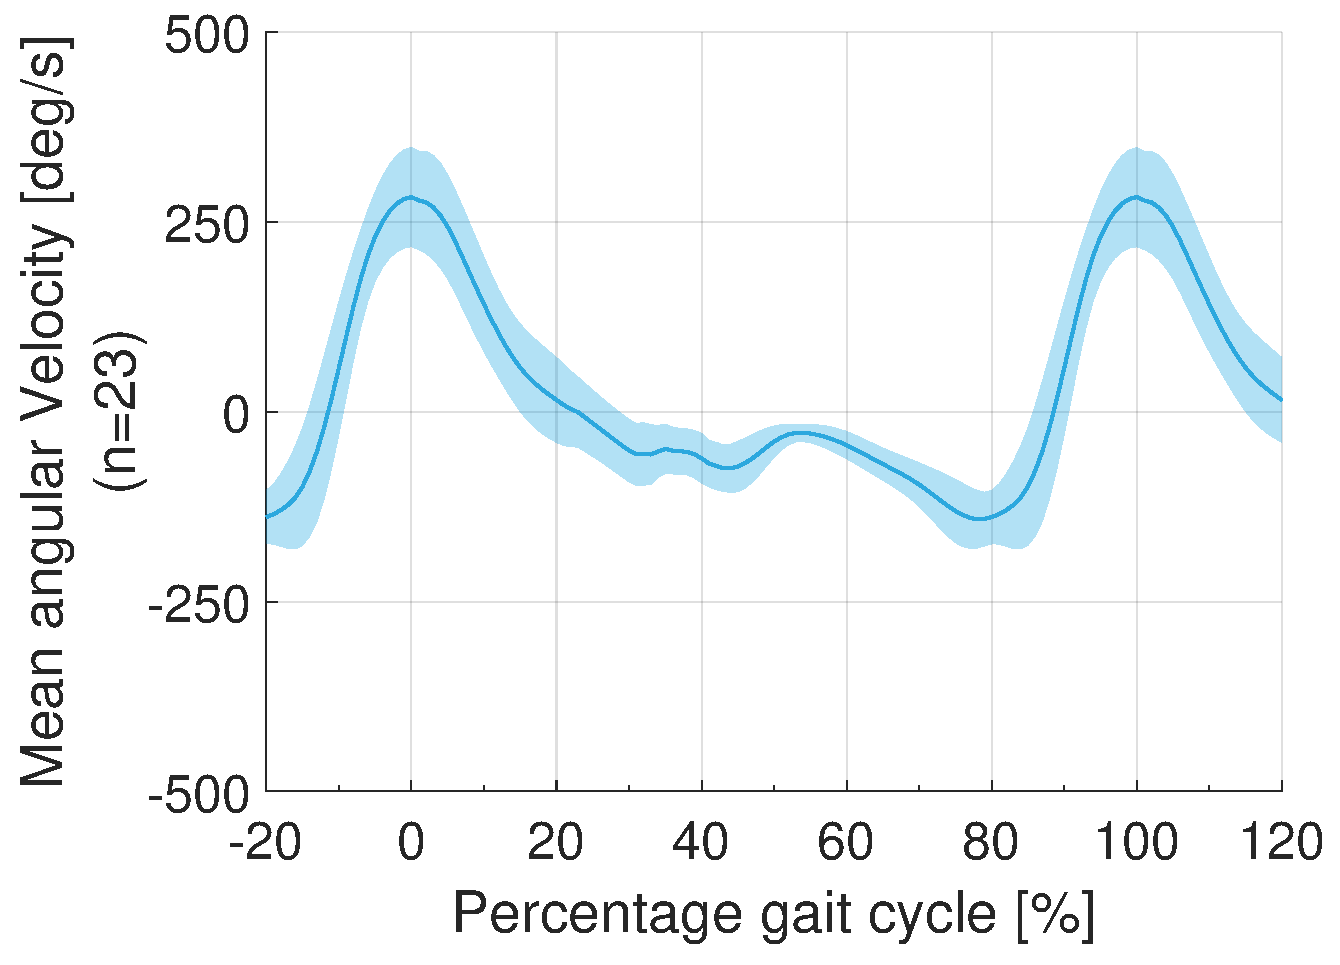
\includegraphics[width=0.275\linewidth]{content/6-Amputee/Gait-Trends/ch6_amputee_gait_trends_l_ankle_gyro_z_activity_stair_down.pdf} &
        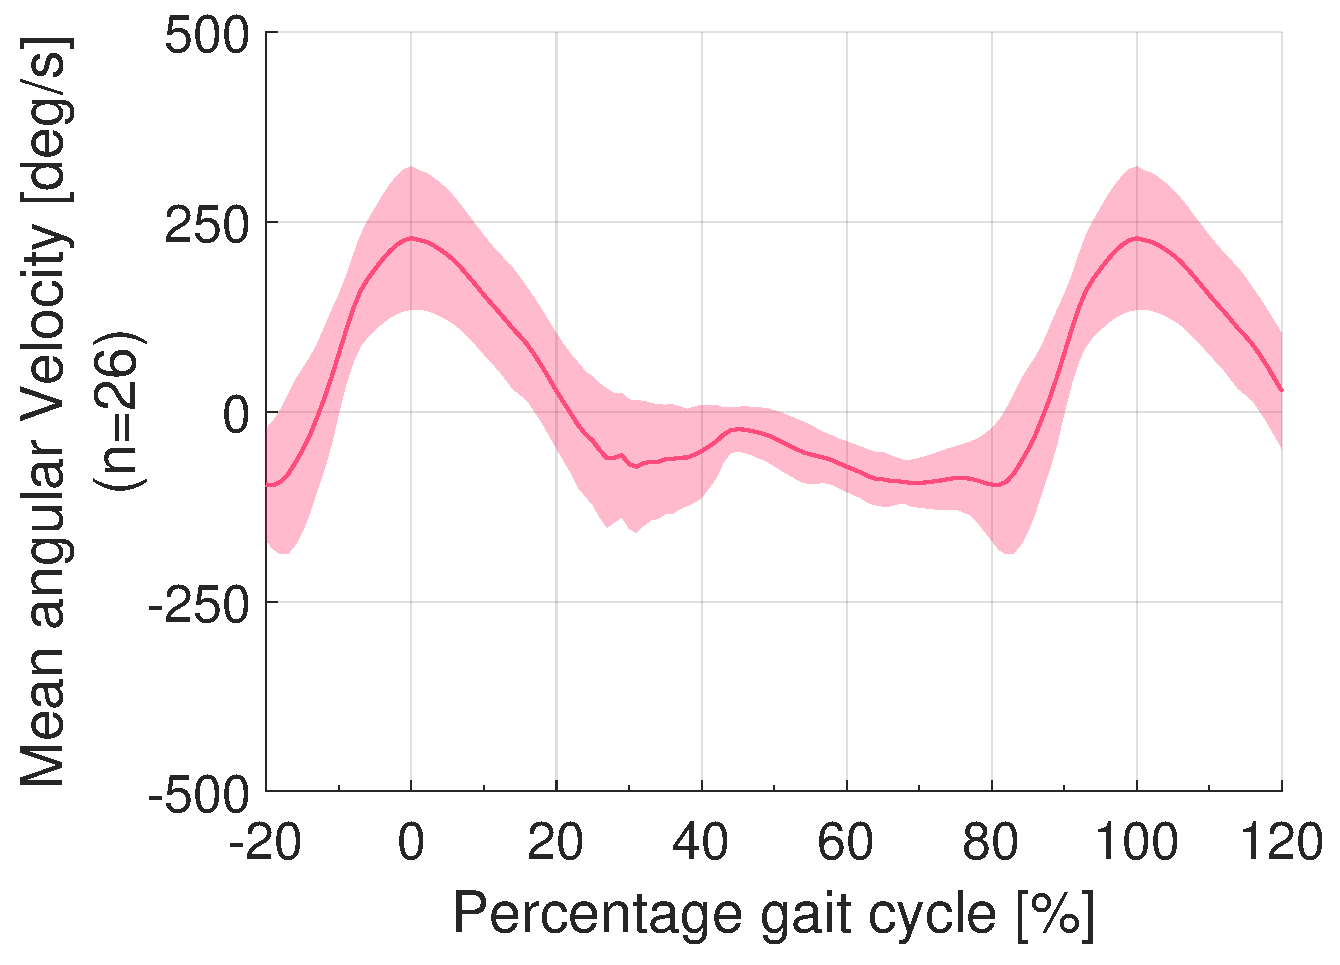
\includegraphics[width=0.275\linewidth]{content/6-Amputee/Gait-Trends/ch6_amputee_gait_trends_r_ankle_gyro_z_activity_stair_down.pdf} \\
    \end{tabular}
    \centering
    % \hspace*{1cm}
\includegraphics[width=0.7\textwidth]{content/6-Amputee/Gait-Trends/Legend.pdf}
    \caption[Angular velocity of the shank in the Saggital Plane for amputee and non-amputee during different activities.]{Angular velocity of the shank in the Saggital Plane for amputee and non-amputee during different activities. The yellow line is for Non-Amputee (Subject 01 Left Ankle); The blue line is the intact limb of  the trans-tibial amputee; The red line is the prosthetic of the trans-tibial amputee. The solid line shows the mean of the steps recorded for each activity. The filled area represents the standard deviation.}
    \label{fig:ch6_amputee_gyro_trends}
\end{figure}

From a visual assessment of plots difference between the intact and amputated limbs can be seen. On the prosthetic side changes in angular velocity are less smooth across all activities. This is particularly visible during early swing (approximately 80\% to 100\% gait cycle) where there is a kink in the upward velocity rise not seen in the intact limb. Changes in angular velocity around strike (approximately 20\%) are also more abrupt.

The intact limb and non amputee are closer but show clear difference during early stance (approximately 20\% to 40\%) with a much lower velocity seen in the intact limb.

This analysis just covers one axis of the gyroscope. Visible difference can also be seen in the other two gyroscope axes and accelerometer. As the intact limb is closer to the non-amputee it should be expected that it will perform more highly than the prosthetic side.

%-----------------------------------------------------------------
\section{Baseline Model Performance}
\label{sec:amputee-baseline}
As before a set of baselines will be produced to determine if the outcome of the personalisation methods results in an improvement in performance. All baselines will be evaluated using the amputee test data sets. The two baselines will be the performance of the general models \acrshort{lmr} and performance of models constructed from only the target amputee's data.

The general models were constructed in the previous chapter from the large source data set of gait data excluding subjects 1, 3 and 9. These are all 32 unit \acrshort{lstm} model. Both the right intact limb and left prosthetic limb of the trans-tibial amputee were tested separately. For the intact limb the general model achieved a classification performance of $74.2\%\pm9.4$. For the amputated Limb the performance was significantly lower at $55.3\%\pm9.6$. The intact limb performs comparable to the non-amputee subjects from the previous study.

Table \ref{tab:ch6-general-model-confusion-matrix} shows the confusion matrix for the general model. The matrix show that the general mode performs poorly on walking and stair descent for both limbs. The performance for stair descent of the prosthetic limb is noteable poor.

\begin{table}[!hbtp]
    \centering
    \caption[Confusion matrix of general models presented with target subject test data]{Confusion matrix of general models presented with target subject test data. Columns represent the prediction labels and the rows represent the real labels. Each value represent the percentage of total predicted labels for that class. (\acrfull{ra}, \acrfull{rd}, \acrfull{sa}, \acrfull{sd})}
    \label{tab:ch6-general-model-confusion-matrix}
    \begin{subtable}{\textwidth}
    \caption{Prosthetic Limb}
    \begin{tabularx}{\textwidth}{ccYYYYYY}
        \noalign{\hrule height 1.5pt}
         & & \multicolumn{6}{c}{\textbf{Predicted Classes}} \\
         \hline
         & & WALK & \glsentryshort{ra} & \glsentryshort{rd} & \glsentryshort{sa} & \glsentryshort{sd} & STOP \\
         \multirow{6}{*}{\rotatebox{90}{\textbf{True Classes}}} 
         & WALK               & 46.6 & 12.8 & 9.0 & 1.7 & 23.1 & 5.9 \\
         & \glsentryshort{ra} & 8.5 & 77.7 & 0.0 & 9.8 & 13.4 & 10.6 \\
         & \glsentryshort{rd} & 26.0 & 6.4 & 91.0 & 0.3 & 33.7 & 2.1 \\
         & \glsentryshort{sa} & 0.0 & 0.4 & 0.0 & 88.1 & 0.0 & 1.0 \\
         & \glsentryshort{sd} & 14.5 & 2.6 & 0.0 & 0.1 & 29.3 & 18.0 \\
         & STOP               & 4.4 & 0.0 & 0.0 & 0.0 & 0.6 & 62.4 \\
         \noalign{\hrule height 1.5pt} \\
    \end{tabularx}
    \end{subtable}

    \begin{subtable}{\textwidth}
    \caption{Intact Limb}
    \begin{tabularx}{\textwidth}{ccYYYYYY}
        \noalign{\hrule height 1.5pt}
         & & \multicolumn{6}{c}{\textbf{Predicted Classes}} \\
         \hline
         & & WALK & \glsentryshort{ra} & \glsentryshort{rd} & \glsentryshort{sa} & \glsentryshort{sd} & STOP \\
         \multirow{6}{*}{\rotatebox{90}{\textbf{True Classes}}} 
         & WALK               & 69.8 & 0.6 & 11.6 & 0.2 & 14.9 & 0.4 \\
         & \glsentryshort{ra} & 14.3 & 97.5 & 0.0 & 21.7 & 7.8 & 4.4 \\
         & \glsentryshort{rd} & 8.5 & 0.0 & 73.4 & 0.0 & 20.7 & 0.0 \\
         & \glsentryshort{sa} & 0.0 & 0.0 & 0.0 & 77.7 & 0.0 & 0.0 \\
         & \glsentryshort{sd} & 0.1 & 1.9 & 15.0 & 0.1 & 55.5 & 0.8 \\
         & STOP               & 7.3 & 0.0 & 0.0 & 0.2 & 1.1 & 94.4 \\
         \noalign{\hrule height 1.5pt} \\
    \end{tabularx}
    \end{subtable}
\end{table}


%------------------------
The second baseline is a set of models trained using only the amputee data. Different quantities of training windows were used to provide performance metrics for a range of data amounts. Figure \ref{fig:ch6-amputee-baseline-bespoke-model} shows the classification performance for both legs when tested with the test data sets. The full results of this experiment can be found in Appendix \ref{chp:tables-of-results} Table \ref{tab:amputee-bespoke-model-table-of-results}. For all models the average number of epochs to train was 7 with a 95\textsuperscript(9)

\begin{figure}[!hbt]
    \centering
    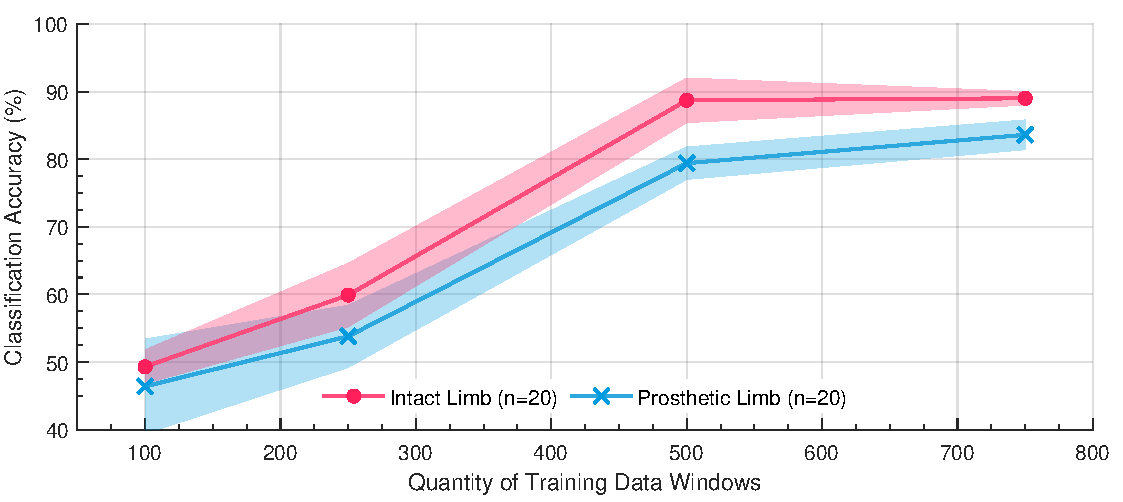
\includegraphics[width=\textwidth]{content/6-Amputee/ch6_baseline_model_accuracy.pdf}
    \caption[Classification accuracy for HAR model using increasing quantities of only amputee target data]{Classification accuracy for HAR model using increasing quantities of only amputee target data. The red line shows the performance of the trained model on the intact limb of a trans-tibial amputee. The blue line shows the performance of the trained model for the prosthetic side. The filled areas represent the standard deviation  (n=4).}
    \label{fig:ch6-amputee-baseline-bespoke-model}
\end{figure}

Figure \ref{fig:ch6-amputee-baseline-bespoke-model} shows performance improving rapidly with increasing training windows levelling out after 500 samples. For all values of training windows the prosthetic limb performing worse than the intact limb. With increasing windows this performance gap between the two limbs widens.

Table \ref{tab:ch6-bespoke-model-confusion-matrix} shows the confusion matrix for both limbs when a bespoke model was trained with 750 training windows. This is markedly better than to the confusion matrix for the general model. This backs up the observations found in literature that general models from non-amputees perform poorly for amputees\cite{Lonini2016, Jamieson2021}. However their are a number of classes across both limbs that perform worse than the general model suggesting the general model contains knowledge that could be used to improve performance.

\begin{table}[hbt]
    \centering
    \caption[confusion matrix for a bespoke amputee \acrshort{lmr} model presented test data]{confusion matrix for a bespoke amputee \acrshort{lmr} model presented with test data. The 32 unit \acrshort{lstm} model was trained with 750 target data window. Columns represent the prediction labels and the rows represent the real labels. Each value represent the percentage of total predicted labels for that class. (\acrfull{ra}, \acrfull{rd}, \acrfull{sa}, \acrfull{sd})}
    \label{tab:ch6-bespoke-model-confusion-matrix}
    \begin{subtable}{\textwidth}
    \caption{Prosthetic Limb}
    \begin{tabularx}{\textwidth}{ccYYYYYY}
        \noalign{\hrule height 1.5pt}
         & & \multicolumn{6}{c}{\textbf{Predicted Classes}} \\
         \hline
         & & WALK & \glsentryshort{ra} & \glsentryshort{rd} & \glsentryshort{sa} & \glsentryshort{sd} & STOP \\
         \multirow{6}{*}{\rotatebox{90}{\textbf{True Classes}}} 
         & WALK               & 68.2 & 0.6 & 42.6 & 0.6 & 0.0 & 0.0 \\
         & \glsentryshort{ra} & 9.7 & 94.0 & 3.8 & 1.4 & 0.5 & 0.0 \\
         & \glsentryshort{rd} & 18.9 & 0.4 & 53.6 & 0.2 & 0.0 & 0.0 \\
         & \glsentryshort{sa} & 0.0 & 0.0 & 0.0 & 79.4 & 0.0 & 0.0 \\
         & \glsentryshort{sd} & 0.0 & 0.0 & 0.0 & 0.0 & 99.5 & 0.0 \\
         & STOP               & 3.2 & 4.9 & 0.0 & 18.4 & 0.0 & 100.0 \\
         \noalign{\hrule height 1.5pt} \\
    \end{tabularx}
    \end{subtable}
% \end{table}
% \begin{table}[t]\ContinuedFloat
%  \caption[]{confusion matrix for a bespoke amputee \acrshort{lmr} model presented with test data. The 32 unit \acrshort{lstm} model was trained with 750 target data window (Cont.).}
    \begin{subtable}{\textwidth}
    \caption{Intact Limb}
    \begin{tabularx}{\textwidth}{ccYYYYYY}
        \noalign{\hrule height 1.5pt}
         & & \multicolumn{6}{c}{\textbf{Predicted Classes}} \\
         \hline
         & & WALK & \glsentryshort{ra} & \glsentryshort{rd} & \glsentryshort{sa} & \glsentryshort{sd} & STOP \\
         \multirow{6}{*}{\rotatebox{90}{\textbf{True Classes}}} 
         & WALK               & 83.1 & 2.6 & 19.3 & 0.0 & 0.0 & 0.0 \\
         & \glsentryshort{ra} & 12.3 & 93.3 & 7.4 & 12.0 & 0.0 & 0.8 \\
         & \glsentryshort{rd} & 3.7 & 0.0 & 72.0 & 0.1 & 3.3 & 0.0 \\
         & \glsentryshort{sa} & 0.0 & 0.0 & 0.0 & 83.6 & 0.0 & 0.0 \\
         & \glsentryshort{sd} & 0.0 & 0.0 & 0.0 & 0.0 & 96.7 & 0.0 \\
         & STOP               & 0.9 & 4.1 & 1.2 & 4.3 & 0.0 & 99.2 \\
         \noalign{\hrule height 1.5pt} \\
    \end{tabularx}
    \end{subtable}
\end{table}

%-----------------------------------------------------------------
\section{Data supplementation} % Are we going to include this?
\label{sec:amputee-supplementation}
The first personalised model technique that will be investigated in data supplementation. This involves supplementing target data with varying amount of data from a general source set to form a large training set. The source data is made up of a larger number of non-amputee subjects. The experiment consisted of mixing 100, 25, 500 and 750 windows of target data with between 100 and 3000 source data windows. Table \ref{tab:ch6-classfication-accuracy-mixed-source-target-right} shows classification performance for all combinations.

\begin{table}[hbt]
    \caption[Table of classification accuracy for amputee test data for a model trained using varying amounts of Source and Target training data]{Table of classification accuracy for amputee test data for a model trained using varying amounts of Source and Target training data. The cell value represents the percentage classification accuracy $\pm\sigma$ $(n=8)$. The highest classification accuracy for each quantity of target windows has been highlighted in bold}
    \label{tab:ch6-classfication-accuracy-mixed-source-target-right}
    \centering
    \begin{subtable}{\textwidth}
    \centering
    \caption{Intact Limb} % Right
    \begin{tabularx}{0.99\textwidth}{cr| *{4}{Y}}
        \noalign{\hrule height 1.5pt}
        & & \multicolumn{4}{c}{\textbf{Target Training Windows}}\\
        & & 100 & 250 & 500 & 750 \\
        \hline
        \multirow{7}{*}{\rotatebox{90}{\parbox{3.4cm}{\centering\textbf{Source Training\\Windows}}}}
& 100 & $0.717{\scriptscriptstyle\pm0.03}$ & $0.682{\scriptscriptstyle\pm0.02}$ & $0.879{\scriptscriptstyle\pm0.02}$ & $0.877{\scriptscriptstyle\pm0.04}$ \\
& 250 & $0.764{\scriptscriptstyle\pm0.04}$ & $0.730{\scriptscriptstyle\pm0.03}$ & $0.883{\scriptscriptstyle\pm0.03}$ & $\mathbf{0.889{\scriptscriptstyle\pm0.01}}$ \\
& 500 & $0.800{\scriptscriptstyle\pm0.04}$ & $0.795{\scriptscriptstyle\pm0.03}$ & $0.875{\scriptscriptstyle\pm0.02}$ & $0.888{\scriptscriptstyle\pm0.02}$ \\
& 750 & $0.815{\scriptscriptstyle\pm0.01}$ & $0.801{\scriptscriptstyle\pm0.02}$ & $0.873{\scriptscriptstyle\pm0.02}$ & $0.881{\scriptscriptstyle\pm0.02}$ \\
& 1000 & $0.801{\scriptscriptstyle\pm0.04}$ & $0.786{\scriptscriptstyle\pm0.03}$ & $\mathbf{0.886{\scriptscriptstyle\pm0.03}}$ & $0.874{\scriptscriptstyle\pm0.02}$ \\
& 1500 & $\mathbf{0.835{\scriptscriptstyle\pm0.03}}$ & $0.794{\scriptscriptstyle\pm0.06}$ & $0.871{\scriptscriptstyle\pm0.01}$ & $0.875{\scriptscriptstyle\pm0.03}$ \\
& 3000 & $0.825{\scriptscriptstyle\pm0.01}$ & $\mathbf{0.826{\scriptscriptstyle\pm0.07}}$ & $0.846{\scriptscriptstyle\pm0.03}$ & $0.863{\scriptscriptstyle\pm0.03}$ \\
        \noalign{\hrule height 1.5pt}\\
        \end{tabularx}
    \end{subtable}
    
    \begin{subtable}{\textwidth}
    \centering
    \caption{Prosthetic Limb} % Left
    \begin{tabularx}{0.99\textwidth}{cr| *{4}{Y}}
        \noalign{\hrule height 1.5pt}
        & & \multicolumn{4}{c}{\textbf{Target Training Windows}}\\
        & & 100 & 250 & 500 & 750 \\
        \hline
        \multirow{7}{*}{\rotatebox{90}{\parbox{3.4cm}{\centering\textbf{Source Training\\Windows}}}}
& 100 & $0.626{\scriptscriptstyle\pm0.05}$ & $0.643{\scriptscriptstyle\pm0.03}$ & $0.855{\scriptscriptstyle\pm0.02}$ & $0.813{\scriptscriptstyle\pm0.04}$ \\
& 250 & $0.714{\scriptscriptstyle\pm0.04}$ & $0.611{\scriptscriptstyle\pm0.02}$ & $0.836{\scriptscriptstyle\pm0.05}$ & $0.843{\scriptscriptstyle\pm0.03}$ \\
& 500 & $0.752{\scriptscriptstyle\pm0.03}$ & $0.729{\scriptscriptstyle\pm0.08}$ & $0.842{\scriptscriptstyle\pm0.02}$ & $0.840{\scriptscriptstyle\pm0.05}$ \\
& 750 & $0.734{\scriptscriptstyle\pm0.06}$ & $0.712{\scriptscriptstyle\pm0.04}$ & $0.848{\scriptscriptstyle\pm0.03}$ & $0.847{\scriptscriptstyle\pm0.02}$ \\
& 1000 & $0.756{\scriptscriptstyle\pm0.02}$ & $0.756{\scriptscriptstyle\pm0.08}$ & $\mathbf{0.875{\scriptscriptstyle\pm0.03}}$ & $\mathbf{0.872{\scriptscriptstyle\pm0.01}}$ \\
& 1500 & $0.734{\scriptscriptstyle\pm0.02}$ & $\mathbf{0.764{\scriptscriptstyle\pm0.05}}$ & $0.869{\scriptscriptstyle\pm0.02}$ & $0.852{\scriptscriptstyle\pm0.02}$ \\
& 3000 & $\mathbf{0.767{\scriptscriptstyle\pm0.02}}$ & $\mathbf{0.764{\scriptscriptstyle\pm0.04}}$ & $0.874{\scriptscriptstyle\pm0.02}$ & $0.849{\scriptscriptstyle\pm0.02}$ \\
        \noalign{\hrule height 1.5pt}\\
    \end{tabularx}
    \end{subtable}
\end{table}

On average each model took 10 epochs 95\textsuperscript(th) percentile of 17. In general the more data used the larger the number of epochs required.

As with before the performance of the prosthetic side is lower than the intact side. All classification accuracies for the prosthetic exceed the general model performance. However for the intact limb the lowest two results for 100 source windows are perform worse than the general model.

For the intact side none of the 500 and 750 target window models exceed the performance on the bespoke models with the same quantity of target windows. For the amputated side all but 750 target, 100 source windows exceed the bespoke model performance.

At lower value a higher quantity of source windows improves performance, at higher target windows less source data is used. At higher values of target data windows the improvement in performance is very minimal, especially for the intact side. This suggests that this method may become less useful the more target data you have.

%-----------------------------------------------------------------
\section{Transfer Learning}
\label{sec:amputee-transfer}
Transfer learning involves using the knowledge captured in an existing model as a starting point to building a personalised model. For this experiment five general models constructed in Chapter \ref{chp:personalisation} were used as the starting point. Varying quantities of target amputee data windows were then used to fine-tune these starting models to personalise them to the amputee. By freezing the different layers of the network attempts to reduce the computation load required to train the model could be made.

In Figure \ref{fig:ch6-amputee-retrain-pre-trained} shows three different experiments in transfer learning. Each trained different layers. The first trained all layers, the just the dense layer, finally just the \acrshort{lstm} layer.

\begin{figure}[!hbtp]
    \centering
    \begin{subfigure}{\textwidth}
        \centering
        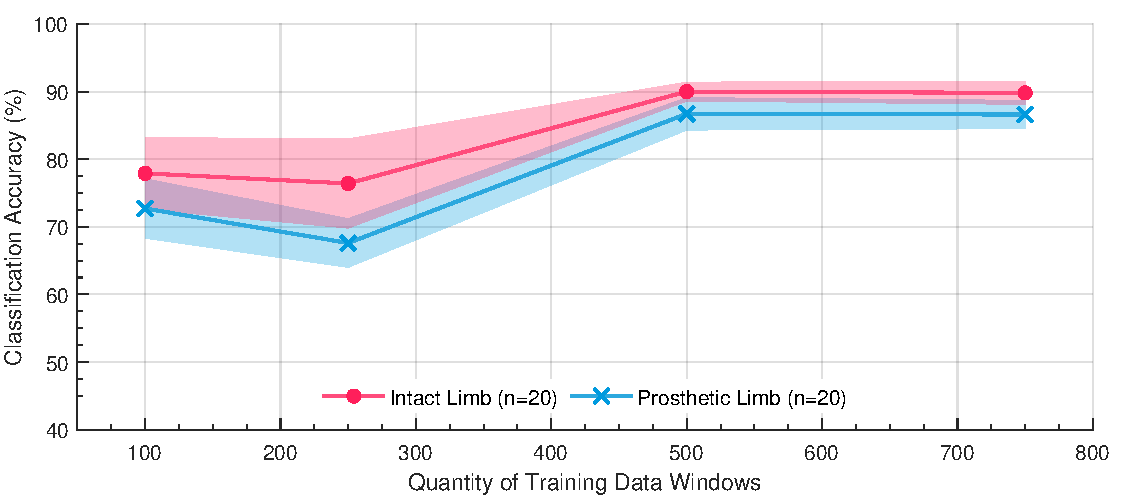
\includegraphics[width=\textwidth]{content/6-Amputee/ch6_pre_trained_model_accuracy.pdf}
        \caption{Fine tuning all layers}
    \end{subfigure}
    \begin{subfigure}{\textwidth}
        \centering
        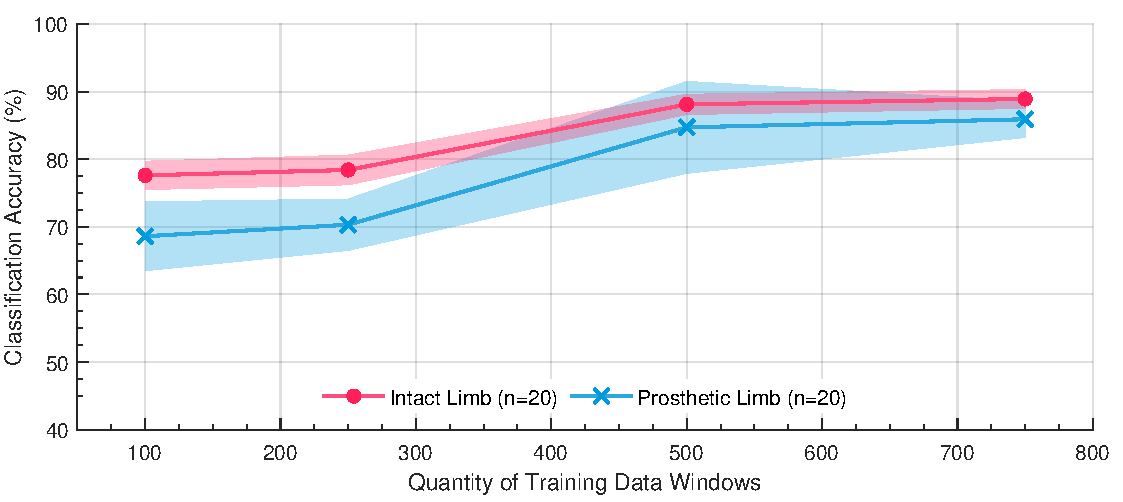
\includegraphics[width=\textwidth]{content/6-Amputee/ch6_frozen_lstm_layer_accuracy.pdf}
        \caption{Fine tuning only the dense layer}
    \end{subfigure}
    \caption[Classification accuracy for re-training a pre-trained model using increasing quantities of amputee target data]{Classification accuracy for re-training a pre-trained model using increasing quantities of amputee target data. The red line shows the performance of the trained model on the intact limb of a trans-tibial amputee. The blue line shows the performance of the trained model for the prosthetic side. The filled areas represent the standard deviation (n=20).}
    \label{fig:ch6-amputee-retrain-pre-trained}
\end{figure}
\begin{figure}[t]\ContinuedFloat
    \centering
    \begin{subfigure}{\textwidth}
        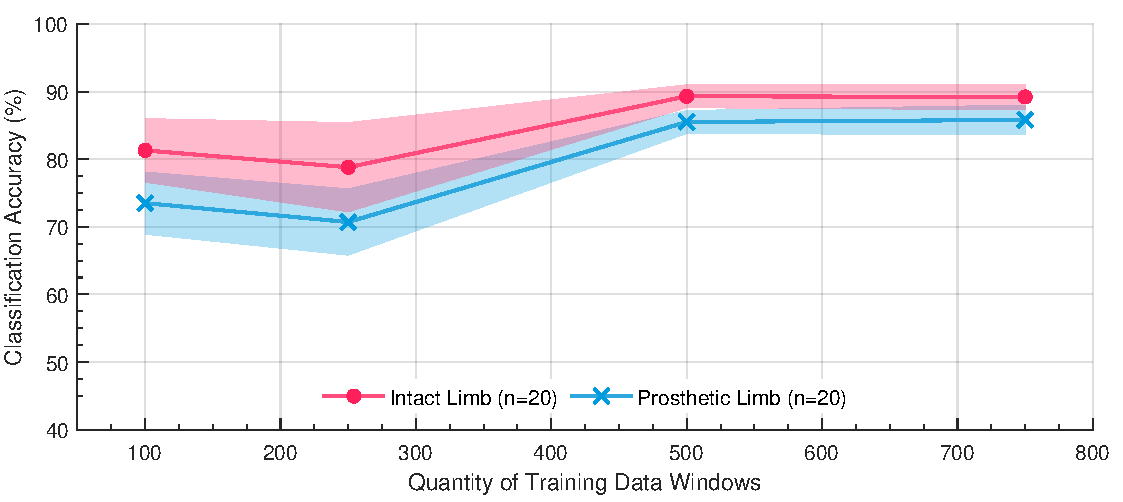
\includegraphics[width=\textwidth]{content/6-Amputee/ch6_frozen_dense_layer_accuracy.pdf}
        \caption{Fine tuning only the \acrshort{lstm} layer}
    \end{subfigure}
    \caption[]{Classification accuracy for re-training a pre-trained model using increasing quantities of amputee target data (Cont.).}
\end{figure}

On average each model took 6 epochs 95\textsuperscript(th) percentile of 10. In general the more data used the larger the number of epochs required.

When training all layers classification performance showed a significant increase in performance over the base general model with only a small amount of target windows. For the prosthetic side with 100 target windows there was a $22\%$ increase in performance over the general model to just under $1\%$ for the intact limb at 750 windows. Transfer learning resulted in an improvement for all setups.

Fine tuning only the dense didn't result in better performance than fine tuning all layers and for the intact limb at 500 and 750 windows was worse than the baseline bespoke model. Using this method resulted in significantly increased standard deviation for the prosthetic limb, although slightly reduced $\sigma$ for the intact limb.

Fine tuning only the \acrshort{lstm} layer gave the better performance for 100 and 250 target windows compared to fine tuning all layer. Performance was a couple of percent better however at the higher two target window quantities performed was approximately a percent worse. Standard deviation remained roughly the same. On balance it therefore showed no improvement over fine tuning all layers.

%-----------------------------------------------------------------
\section{Discussion and Conclusions}
\label{sec:amputee-discussion}
The work in this chapter set out to investigate it the personalisation methods for a \acrshort{lmr} classifier developed in Chapter \ref{chp:personalisation} were applicable to a amputee with a severe gait impediment. To achieve this a set of comparable data was collected from a trans-tibial amputee. This was then used to repeat the previous experiments for the amputee subject.

% SUMMARY TABLE OF PERFORMANCE FOR EACH METHOD
\begin{table}[]
    \centering
    \begin{tabular}{c|c}
         &  \\
         & 
    \end{tabular}
    \caption{Caption}
    \label{tab:my_label}
\end{table}

Jamieson and Lonini both suggested that the direct use of a general model trained using only non-amputee data would not perform adequately for a person with gait impairments\cite{Lonini2016, Jamieson2021}. This was borne out in the results as when data from the prosthetic limb is classified it only achieved a classification accuracy of $55.3\%$. However when data from the amputee's intact limb was use classification performance was much higher. For the test subject they have a significant asymmetry in their gait however the intact side matches much more closely to the source non-amputee's gait.

Both the data supplementation and transfer learning approaches resulted in an improvement over the baseline classifiers. The differences observed in the previous chapter were again shown. The quantity of source data required for data supplementation was hard to predict and only training specific layers for transfer learning resulting in minimal changes. As before the transfer learning performance appeared to perform more consistently and required significantly less computing resources to train.

The overall performance of both the bespoke model and personalised models at 500 and 750 training windows was significantly higher than seen in the previous chapter. They also looked more likely to be levelling off in performance. There are two likely reasons for this. First a much smaller testing set was used so the trained model was tested with a much narrower range of environments. Secondly all the amputee data was collected at a single site and therefore the training data is likely to include environments also seen in the test set. The division of episode for stairs would also have the same effect. 

Further to as unfortunately data for only one amputee was collected it is not possible to say whether these methods are more generally applicable. To test the results further both more amputees and more data per amputee is required. 

In the previous chapter a method for improving data supplementation suggested was data grouping. It's unlikely to be successful in this scenario due to the likely difficulty in find subjects with a similar gait to an amputee. However their may be potential in including more persons with gait impairments to improve the networks ability to adapt. This is a potential are for further research.

There was no literature found investigating the classification performance difference between the two lower limbs of a amputee or other person with asymmetric gait. The results consistently showed that classification of the intact limb produced higher accuracies. This could be an interesting area of research for improving performance of classifier using both sides of the body. An form of ensemble network could be a good candidate for this.

Overall these methods show promise in the area of amputee gait classification. Further research is required in this area to exploit to potentials for using non-amputee data to reduce data requirements for amputees.


% WHY IS THIS USEFUL/HOW COULD IT BE EXPLOITED